\section{Deployment View}

The following Deployment Diagram describes the execution architecture of the software system; it includes nodes such as hardware or software execution environments and the middleware connecting them. In other words, this kind of diagram describes the physical deployment of information generated by the software program on hardware components: the information that the software generates is called an artifact. The purpose of this section is to visualize how the system will be physically deployed on the hardware. As can be clearly seen from the figure, the system is divided into three tiers:
\begin{itemize}
	\item\textbf{Presentation Tier}: it contains the presentation logic for Customers and Store Managers. In particular:
		\begin{itemize}
			\item\textbf{Smartphone}: Customers exploit the \textbf{CLupMobileApp} for accessing the booking and line-up services.
			\item\textbf{PC/Laptop}:  Store Managers have access to their services through a simple \textbf{WebApp}.
		\end{itemize}
	All the operations both on MobileApp and on WebApp side are possible through the communication via server, that retrieves all kind of data needed.
	\item\textbf{Application Tier}: the main logic of the application will be deployed here. In particular, it comprises:
		\begin{itemize}
			\item\textbf{Web Server}: this component communicates and serves the WebApp through the HTTPS protocol; it is mainly used for static requests, and so, when dynamic contents are required, it contacts the Application Server using JavaRMI for further processing.  
			\item\textbf{Application Server}: this component contains the actual application logic: it handles all the requests and provides the appropriate answers for all the offered services. This server can communicate directly with the MobileApp through HTTPS protocol; moreover, it handles also some requests of the WebApp that the Web Server cannot satisfy and that, for this reason, are forwarded to the Application Server: in this case, the two servers communicate exploiting JavaRMI. If needed, this component could be replicated in order to avoid a single point of failure and to guarantee better performances avoiding a bottleneck effect. %In generale, il WebServer è un "subset" dell' ApplicationServer
		\end{itemize}
	\item\textbf{Data Tier}: will store all the persistent data for the Customers and StoreManagers, such as their usernames and passwords, as well as the Bookings, Line-ups and all the other kind of informations useful for the application. In particular, this tier contains the \textbf{DatabaseServer}, which communicates with the ApplicationServer through the standard protocol TCP/IP and provide access to the physical database.\\
\end{itemize}
In the system, also other two kind of devices are exploited:
	\begin{itemize}
			\item\textbf{Firewall}: this device monitors incoming and outgoing network traffic and permits or blocks data packets based on a set of security rules. Its purpose is to establish a barrier between the internal network and incoming traffic from external sources in order to block malicious traffic like viruses and hackers.
			\item\textbf{Load Balancer}: it distributes the workload across multiple servers to increase capacity; this is needed beacuse CLup is an application which, hopefully, will be used by a very huge amount of users. Moreover, this device can improve the reliability trying to avoid the overload of any single server: this is fundamental because grocery shoppings are one of the most essential needs of the people. 
	\end{itemize}


\begin{figure}[H]
\centerline{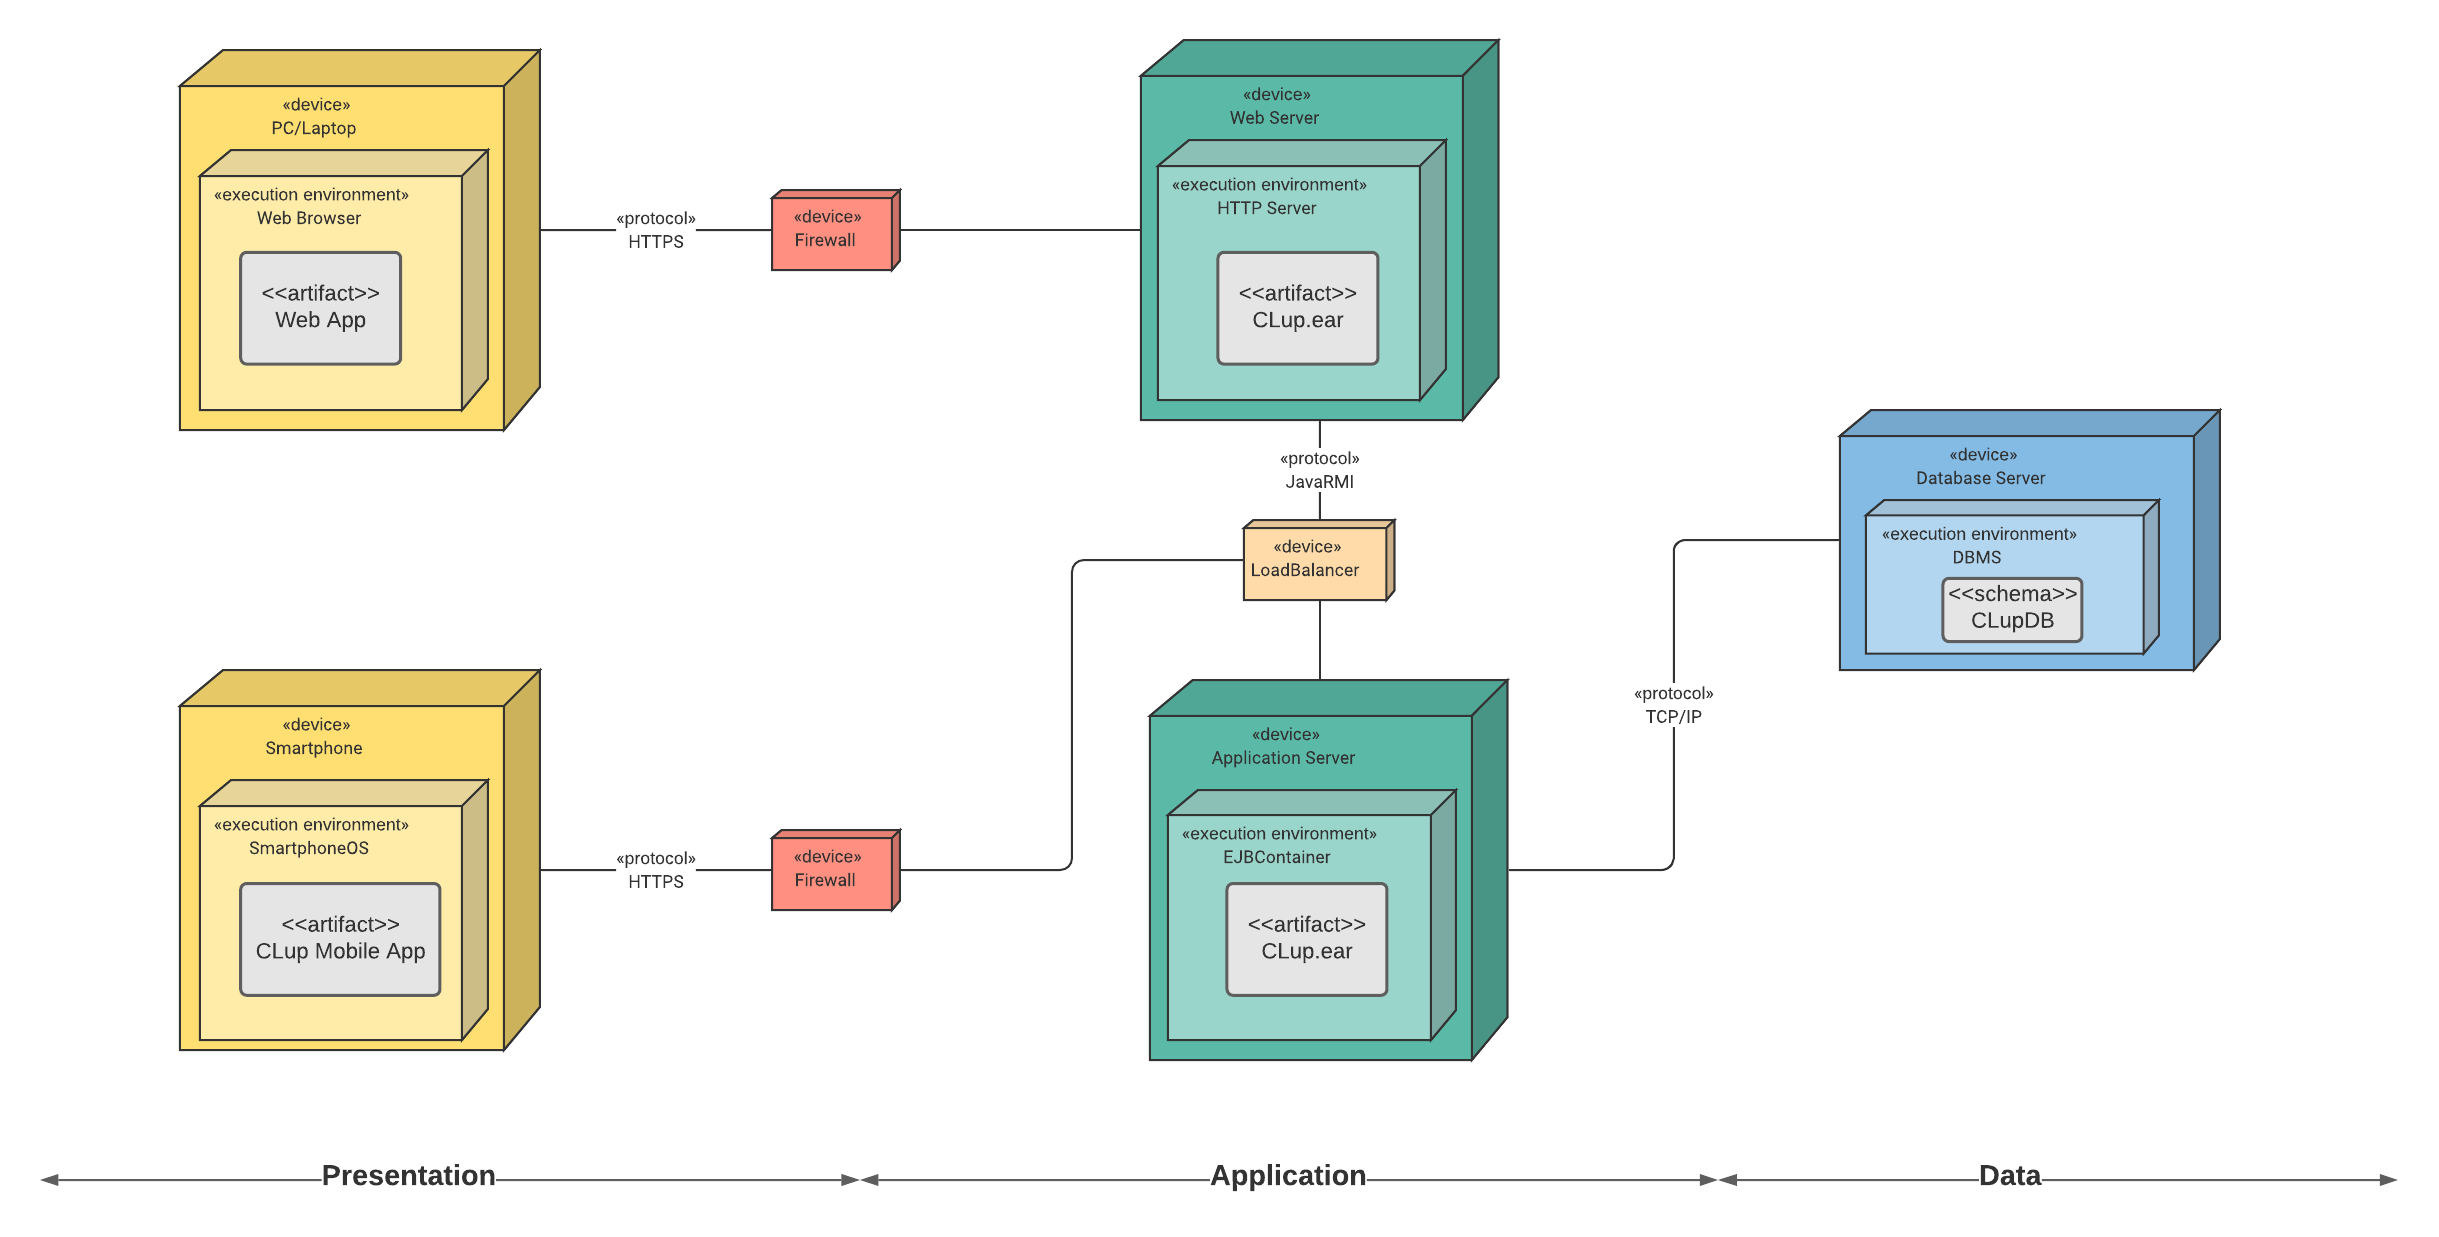
\includegraphics[scale=0.5]{./Deplo}}
\caption{Deployment Diagram}
\end{figure}



 
 